%=== CHAPTER THREE (3) ===
%=== (Actual work done and contribution, including literature survey) ===

\chapter{Research Methodology}
\begin{spacing}{2.0}
	%\setlength{\parskip}{0.2in}
	%  (Actual work done and contribution, including literature survey)


	\section{Chapter Introduction}

	% Mention the aim of the study and reference the research questions, using the SOI.

	% Create mini summary of selected research papers and notes to better align the research questions and methodology with the literature review.

	% \section{Nature of Research}
	% % Should I discuss this in its own section, or just include my own notes and split it in the introduction and especiialy discuss it % in the data collection,
	% % as it is more relevant to the data collection and evaluation sections and is covered more in depth there.
	%    \subsection{}

	% Should this just be called the Research Pipeline?
	\section{Conceptual Framework}

	Figure \ref{fig:pipeline} outlines the methodology pipeline for this study's research, with it being divided into 4 major sections.
	The first section consisted of decided on the prerequisites and tools required for the development of the prototype, along with developing the
	traditional game mechanics and State Machine opponent. The second section consisted of setting up the training scene and Unity mL-Agents plugin,
	training, and evaluating the RL-Agent. The third section involved developing the data collection and developing the DDA system using behaviour-trees,
	which were decided over the other options due to their ease-of-use, and how well they are at representing the AI's decision making process.
	Finally, the prototype was evaluated by the participants, with the data collected being analysed and compared to previous research to answer the research questions.

	\begin{figure}[ht]
		\centering
		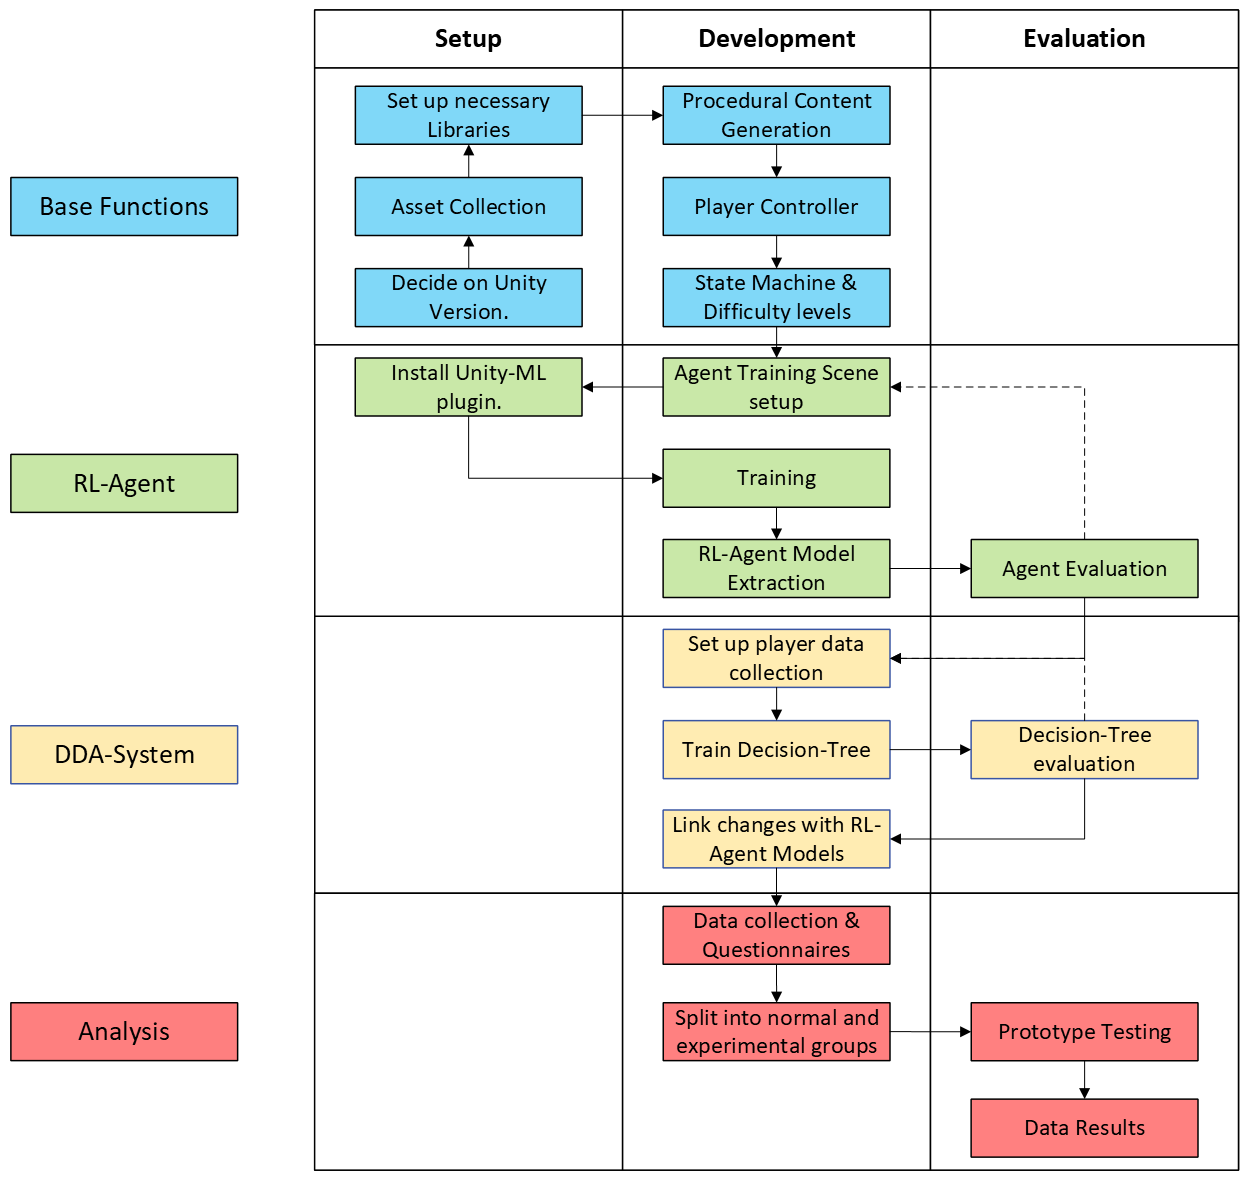
\includegraphics[width=5in, fbox]{Figures/ResearchPipeline.png}
		\caption{Diagram representing the methodology pipeline.}
		\label{fig:pipeline}
	\end{figure}

	\section{Prerequisites and Tools}

	Before starting development on the prototype, a github repository for the project was created, and Jetbrains Rider was used as the IDE for the project.
	The prototype was developed using Unity 6000.0.31f1, and utilised several Unity packages, assets and plugins, which are listed below:

	% Do I list them here or reference an appendix?

	Along with the built-in Unity packages, the project also used the Unity ML-Agents package which was cloned off the Unity ML-Agents github repository, and the Unity ML-Agents Toolkit, which was cloned off the Unity ML-Agents Toolkit github repository,
	and then imported into the project as a Unity package along with the ML-Agents Extensions packages. The version of ML-Agents used in the prototype
	was version 22, the latest version at the time of development.

	\section{Prototype Outline \& Implementation}

	% Likely will need to split this into an outline, with the State Machine being a subsection, and the RL-Agent and DDA system being their own sections.

	A Prototype game was developed to implement and test the RL-Agent and DDA system for their effectiveness in creating a dynamic and adaptive game experience.
	The core gameplay will consists of traversing the game world in a third person perspective, with the goal to mine and deposit as many ores as possible.
	There are 3 main mechanics which for the core gameplay loop of the game, the scoring system, the mining system, and the inventory system. The mining system is responsible for the player's ability to mine ores,
	the scoring system is responsible for tracking the player's score and awarding them points based on the types or ores deposited, and the inventory system is responsible for forcing the player to carefully
	think about their inventory space and which ores to mine and when to go deposit. The ores and terrain are procedurally generated, with some small obstacles which can force the player to take a slightly longer path.

	\begin{figure}[ht]
		\centering
		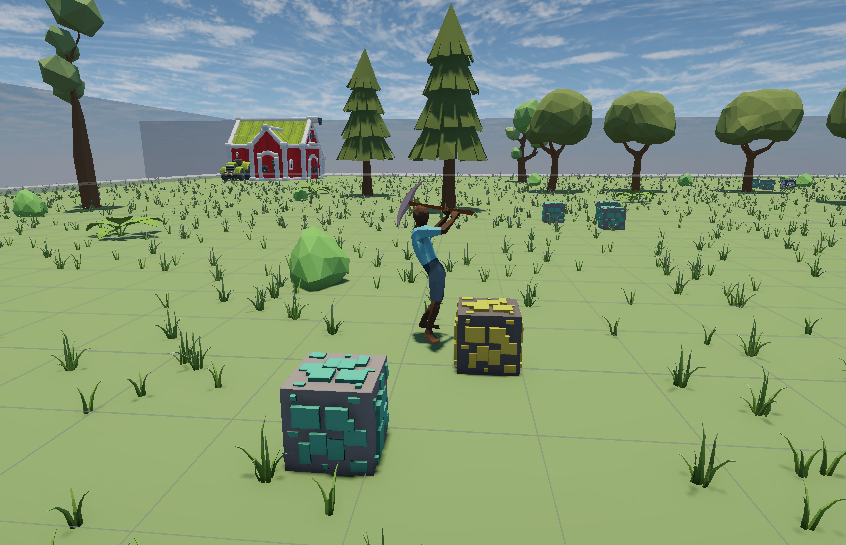
\includegraphics[width=5in, fbox]{Figures/Gameplay.png}
		\caption{Screenshot of gameplay showing the gathering of resouces.}
		\label{fig:gameplay}
	\end{figure}

	The main challenge the player will face is the AI opponent which has the same goal and capabilities of the player. The objective for both of them is to gather as many points as possible before the game ends.
	If the player has more points at the end, they win, if its the same, it is a draw, and if the AI has more points, the player loses. The AI opponent will be different for each stage of the test, with the first
	being a State Machine, and the second being an RL-Agent. More information regarding the test stages and how data will be gathered and analysed will be discussed in a later section.

	\subsection{Ores}

	There are three types of ores in the game, Copper, Silver, and Gold. Each ore is visually distinct, as can be seen in Figure \ref{ores} and have a different chance of spawning, as listed in Table \ref{ore_chance_table}.

	\begin{figure}[ht]
		\centering
		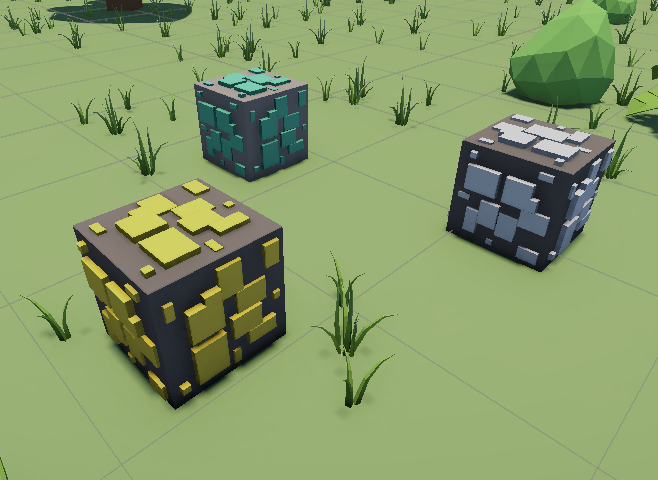
\includegraphics[width=5in, fbox]{Figures/Ores.png}
		\caption{Screenshot showing the different ores.}
		\label{fig:ores}
	\end{figure}

	\begin{table}[ht]
		\centering
		\renewcommand{\arraystretch}{1.2} % Adjust row spacing
		\setlength{\tabcolsep}{8pt} % Adjust column spacing
		\begin{tabular}{|c|c|c|c|}
			\hline
			\textbf{Difficulty} & \textbf{Copper Spawn \%} & \textbf{Silver Spawn \%} & \textbf{Gold Spawn \%} \\
			\hline
			Easy                & 60\%                     & 30\%                     & 10\%                   \\
			\hline
			Medium              & 70\%                     & 25\%                     & 5\%                    \\
			\hline
			Hard                & 75\%                     & 20\%                     & 5\%                    \\
			\hline
		\end{tabular}
		\caption{Chance of spawning for each ore.}
		\label{ore_chance_table}
	\end{table}

	They also take different amounts of time to mine, inventory space, and points awarded when deposited, as listed in Table \ref{ore_table}.

	\begin{table}[ht]
		\centering
		\renewcommand{\arraystretch}{1.2} % Adjust row spacing
		\setlength{\tabcolsep}{8pt} % Adjust column spacing
		\begin{tabular}{|c|c|c|c|}
			\hline
			\textbf{Resource Type} & \textbf{Score} & \textbf{Mining Time (swings)} & \textbf{Inventory Space Taken} \\
			\hline
			Copper                 & 2              & 3                             & 1                              \\
			\hline
			Silver                 & 5              & 5                             & 3                              \\
			\hline
			Gold                   & 10             & 8                             & 5                              \\
			\hline
		\end{tabular}
		\caption{Ore statistics.}
		\label{ore_table}
	\end{table}

	\subsection{Traditional State Machine}

	The State Machince will be a simple AI opponent using the Unity navmesh system to navigate the game world. The AI will have 3 states, a mining state, a depositing state, and a travelling state.
	After completing a task, the AI will use a Physics OverlapSphere to search for the best ore within the vicinity, and once the best option is found, the AI will navigate to the ore and mine it.
	The speed at which the AI travels, and the radius it searches for ores will be adjusted based on the difficulty selected, allowing for a faster and more effective opponent on higher difficulties.
	Once the inventory is full, the AI will navigate to the closest deposit point to deposit the ore and gain points.

	\subsection{RL Agent}

	The Reinforcment Learning Agent will be trained using the Unity ML-Agents plugin, and will use Proximal Policy Optimisation (PPO) as the training algorithm, since it is the most commonly used algorithm due to
	its effectiveness at training agents in complex and continuously changing environments, the main RL training algorithm for the Unity ML-Agents framework, and the one used in the works done by \cite{grech_creating_2023},
    \cite{bin_ramlan_implementation_2021}, \cite{berta_development_2024}, and \cite{raut_unity_2024}.
	The agent will then be placed instead of the State-Machine as the opponent the player will face. More information on the training and evaluation will be discussed in a later section.

	\subsection{DDA System}

	This section will be created over time while the prototype and DDA system are being developed and tested.

	\section{RL-Agent opponent}

	\subsection{Agent Observations}

	To understand the game enviroment, the agent is supplied with several variables to observe via the Unity ML-Agents plugin. These variables are all normalised numerical values between 0 and 1, and are as follows:

	\begin{itemize}
		\item The type of ore currently being obesrved.
		\item How much of the inventory the ore will take up.
		\item The agents normalised position from the ore.
		\item The player's normalised position from the ore.
		\item The deposit point's normalised position from the ore.
		\item The normalised amount of inventory space left.
		\item The normalised amount of time left.
	\end{itemize}

	\begin{figure}[ht]
		\centering
		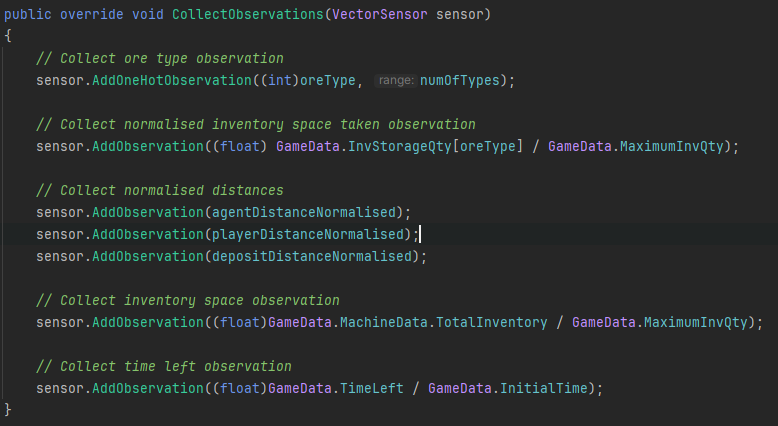
\includegraphics[width=5in, fbox]{Figures/Observations.png}
		\caption{Screenshot showing the Agent's observations.}
		\label{fig:observations}
	\end{figure}

	\subsection{Agent Decisions \& Actions}

	The Agent has 3 decisions it can make, and 2 actions it can take. The decisions are between travelling to and mining the ore being observed, travelling to the deposit point, or observing the next ore.
	The travel to \& mining action involves setting the ore's position as the NavmeshAgent's destination, waiting until the agent arrives, and then mine the ore. Sometimes due to obstacles and the agent's pathfinding,
	the agent may get stuck, which the program will detect very quickly by requesting the agent to decide on another ore. While this is not ideal, it is an uncommon bug with the NavmeshAgent.
	The other action the agent can take is travelling to the deposit point, which acts similarly to the travel to \& mining action, but instead of mining, the agent will just observe and make another decision once it arrives.

	% NOTE: Add flowchart of the agent's decision making process here.

	% TODO: Expand on the agent's observation and decision making.

	\subsection{Agent Rewards \& Penalties}

	A simple reward and penalty system was used to train the agent, since the enviroment is simple and the agent's goal is clear. The focus was on rewarding the agent for mining and depositing ores,
	and penalising them for travelling for too long.

	% TODO: Show the final rewards and penalty systems that will be used

	\subsection{Agent Training}

	\subsection{Model Selection \& Evaluation}

	\section{Data Collection}

	% Should the participants come before the type of data?
	% Should i mention the tests and how the data will be gathered after the sub sections, and use the sub sections to explain the type of data, why it is being collected and who it is being collected from, or should this come before?

	It was decided to use a mixed-methods approach for the evaluation of the prototype, with the majority of the data being quantitative.
	This was chosen to better match \cite{grech_creating_2023} \& \cite{mercieca_evaluating_2023}'s approaches, allowing for an in-depth comparison and analysis of results,
	while allowing for a more detailed understanding of the player's experience and recommendations. Quantitative data will be collected through Unity Analytics, allowing data to be extracted from gameplay sessions,
	as well as close ended questionnaires. Quantitative data will be collected through open ended questions in the questionnaire.

	\subsection{Quantitative Data}

	To better understand the performance of the agent and DDA system against a human player, and to compare the two against State Machines, important statistics throughout the game will be tracked, and saved to a database.
	This data will include the player and enemy action logs, the game summary, and the performance summary.

	\subsubsection{Player and Enemy Action Logs}

	These logs, as seen in \ref{fig:logs} will show all note-worthy actions taken by the player and the enemy, detailing the time, action and any relelvant information, such as the time left and score, and will be shown in chronological order.
	This data will be used to analyse the player's and enemy's behaviour and decision making throughout the game.

	\subsubsection{Game \& Perfomance Summary}

	The game summary will show some of the less note-worthy actions taken by the player and enemy, such as time spent mining and travelling. It will also show the final score and the difficulty selected.
	Due to the DDA system in place, some of the statistics will include logs of difficulty adjustments, and the final difficulty the DDA system selected. The performance summary will be used to capture the
	game's performance by tracking metrics such as frame-rate, CPU Usage and memory usage.

	\subsection{Qualitative Data}

	To better understand the player's experience, as well as some pain points of the game, the questionnaires will have some open ended questions, asking the player to better describe their experience,
	and to provide feedback and any recommendations that they might have. This data will help expand upon the metrics gathered from the quantitative data, and will be used to better answer the research questions.

	\subsection{Participants}

	To really gauge the effectiveness of RL-Agents and DDA systems in creating a dynamic and adaptive experience, a large diverse group of participants will be required.
	% TODO: Add more info about the number of participants and such instead of saying large and diverse.
	By having players of different ages and experience, the data collected will be more varied and allow for a more in-depth analysis of the data. This is inline with the research being conducted, as the goal is to
	identify places where AI is worth implementing, such as more difficult competitive games, or games with a more casual audience.

	\subsection{Tests}
	% Mention that they will agree to the notice found at the end of the SOI
	The tests will be conducted in two stages. First, a close-ended questionnaire will be taken by the participants to gather basic information anonymously, such as age and gaming experience. Once complete,
	the participants will be split into two groups, ensuring that both groups have a similar distribution of age and experience, and they will both play the traditional segment of the prototype,
	with traditional difficulty settings and a State Machine as the opponent. In the second stage, the first group will then play against the RL-Agent, whereas the second group will play against the RL-Agent
	with the DDA system in place. After each playtest, the participants will be given a questionnaire to describe their experience and provide feedback, with both closed and open-ended questions. As mentioned earlier,
	data from the playtests will also be gathered through Unity Analytics.

	\section{Evaluation}

	The data collected from the playtests and questionnaires will be analysed and cross-referenced to find any patterns or correlations between the data.
	The quantitative parts of the data will be analysed using T-Test analysis, and the qualitative data will be analysed using thematic analysis. The results will then be compared to previous research,
	and then be used to answer the research questions, and to prove or disprove the hypothesis.

	\section{Chapter Overview}

	%=== END OF CHAPTER THREE ===
\end{spacing}
\newpage
